\documentclass[11pt,letterpaper]{article}

\addtolength{\oddsidemargin}{-.875in}
\addtolength{\evensidemargin}{-.875in}
\addtolength{\textwidth}{1.75in}

\addtolength{\topmargin}{-.875in}
\addtolength{\textheight}{1.75in}

\usepackage[utf8]{inputenc}
\usepackage{caption} % for table captions
\usepackage{amsmath} % for multi-line equations and piecewises
\DeclareMathOperator{\sign}{sign}
\usepackage{graphicx}
\usepackage{relsize}
\usepackage{xspace}
\usepackage{verbatim} % for block comments
\usepackage{subcaption} % for subfigures
\usepackage{enumitem} % for a) b) c) lists
\newcommand{\Cyclus}{\textsc{Cyclus}\xspace}%
\newcommand{\Cycamore}{\textsc{Cycamore}\xspace}%
\newcommand{\deploy}{\texttt{d3ploy}\xspace}%
\newcommand{\Deploy}{\texttt{D3ploy}\xspace}%
\usepackage{tabularx}
\usepackage{color}
\usepackage{multirow}
\usepackage{float}
\usepackage[acronym,toc]{glossaries}
\newacronym{ANL}{ANL}{Argonne National Laboratory}
\newacronym{B4C}{B4C}{boron carbide}
\newacronym{BC}{BC}{boundary condition}
\newacronym{BOC}{BOC}{beginning of equilibrium cycle}
\newacronym{BSD}{BSD}{Berkeley Software Distribution}
\newacronym{BWR}{BWR}{Boiling Water Reactor}
\newacronym{CAISO}{CAISO}{California ISO}
\newacronym{CEA}{CEA}{Commissariat a l'Energie Atomique}
\newacronym{CFD}{CFD}{computational fluid dynamics}
\newacronym{CO2}{CO$_2$}{carbon dioxide}
\newacronym{CR}{CR}{control rod}
\newacronym{CRP}{CRP}{Coordinated Research Project}
\newacronym{CZP}{CZP}{Cold Zero Power}
\newacronym{DCC}{DCC}{depressurized conduction cool-down}
\newacronym{DOE}{DOE}{Department of Energy}
\newacronym[\glslongpluralkey={degrees of freedom}]{DoF}{DoF}{degree of freedom}
\newacronym{EOC}{EOEC}{end of equilibrium cycle}
\newacronym{FCEV}{FCEV}{Fuel Cell Electric Vehicle}
\newacronym{FDM}{FDM}{Finite Difference Method}
\newacronym{FEM}{FEM}{Finite Element Method}
\newacronym{FVM}{FVM}{Finite Volume Method}
\newacronym{FSV}{FSV}{Fort St. Vrain}
\newacronym[\glslongpluralkey={greenhouse gases}]{GHG}{GHG}{greenhouse gas}
\newacronym{GRS}{GRS}{Gesellschaft für Anlagen und Reaktorsicherheit}
\newacronym{H2}{H$_2$}{hydrogen}
\newacronym{He}{He}{helium}
\newacronym{HFP}{HFP}{Hot Full Power}
\newacronym{HPCC}{HPCC}{high pressure conduction cool-down}
\newacronym{HTE}{HTE}{High-Temperature Electrolysis}
\newacronym{HTGR}{HTGR}{High-Temperature Gas-Cooled Reactor}
\newacronym{HTR}{HTR}{High Temperature Reactor}
\newacronym{HTTR}{HTTR}{High Temperature Test Reactor}
\newacronym{HZDR}{HZDR}{Helmholtz-Zentrum Dresden-Rossendorf}
\newacronym{IAEA}{IAEA}{International Atomic Energy Agency}
\newacronym{icap}{iCAP}{Illinois Climate Action Plan}
\newacronym{INL}{INL}{Idaho National Laboratory}
\newacronym{IPyC}{IPyC}{inner pyrolytic carbon}
\newacronym{JFNK}{JFNK}{Jacobian-Free Newton-Krylov}
\newacronym{KAERI}{KAERI}{Korea Atomic Energy Research Institute}
\newacronym{Keff}{K$_{eff}$}{multiplication factor}
\newacronym{LBP}{LBP}{Lumped Burnable Poison}
\newacronym{LGPL}{LGPL}{Lesser GNU Public License}
\newacronym{LOCA}{LOCA}{loss of coolant accident}
\newacronym{LPCC}{LPCC}{low pressure conduction cool-down}
\newacronym{LTE}{LTE}{Low-Temperature Electrolysis}
\newacronym{LWR}{LWR}{Light Water Reactor}
\newacronym{MC}{MC}{Monte Carlo}
\newacronym{MHTGR}{MHTGR}{Modular High-Temperature Gas-Cooled Reactor}
\newacronym{MOC}{MOC}{middle of equilibrium cycle}
\newacronym{MOOSE}{MOOSE}{Multi-physics Object-Oriented Simulation Environment}
\newacronym{MPI}{MPI}{Message Passing Interface}
\newacronym{MSR}{MSR}{Molten Salt Reactor}
\newacronym{MTD}{MTD}{Champaign-Urbana Mass Transit District}
\newacronym{NEA}{NEA}{Nuclear Energy Agency}
\newacronym{NEM}{NEM}{Nodal Expansion Method}
\newacronym{NGNP}{NGNP}{Next Generation Nuclear Power}
\newacronym{NRC}{NRC}{Nuclear Regulatory Commission}
\newacronym{NSC}{NSC}{Nuclear Science Committee}
\newacronym{OECD}{OECD}{Organisation for Economic Co-operation and Development}
\newacronym{OPyC}{OPyC}{outer pyrolytic carbon}
\newacronym{ORNL}{ORNL}{Oak Ridge National Laboratory}
\newacronym{OS}{OS}{Operator-Splitting}
\newacronym{PBMR}{PBMR}{Pebble Bed Modular Reactor}
\newacronym{PDE}{PDE}{Partial Differential Equation}
\newacronym{PMR}{PMR}{Prismatic Modular Reactor}
\newacronym{PV}{PV}{photovoltaics}
\newacronym{RSC}{RSC}{Reserve Shutdown Control}
\newacronym{RSD}{RSD}{Relative Standard Deviation}
\newacronym{SD}{SD}{Standard Deviation}
\newacronym{SI}{SI}{Sulfur-Iodine}
\newacronym{SiC}{SiC}{silicon carbide}
\newacronym{SMR}{SMR}{Small Modular Reactor}
\newacronym{SNU}{SNU}{Seoul National University}
\newacronym{SOEC}{SOEC}{Solid Oxide Electrolysis Cells}
\newacronym{TIP}{TIP}{transverse integration procedure}
\newacronym{TRISO}{TRISO}{Tristructural Isotropic}
\newacronym{UIUC}{UIUC}{University of Illinois at Urbana-Champaign}
\newacronym{UNIST}{UNIST}{Ulsan National Institute of Science and Technology}
\newacronym{UK}{UK}{United Kingdom}
\newacronym{UMICH}{UMICH}{University of Michigan}
\newacronym{US}{US}{United States}
\newacronym{VHTR}{VHTR}{Very High Temperature Gas Cooled Reactor}
%\newacronym{<++>}{<++>}{<++>}
%\newacronym{<++>}{<++>}{<++>}

\definecolor{bg}{rgb}{0.95,0.95,0.95}
\newcolumntype{b}{X}
\newcolumntype{f}{>{\hsize=.15\hsize}X}
\newcolumntype{s}{>{\hsize=.5\hsize}X}
\newcolumntype{m}{>{\hsize=.75\hsize}X}
\newcolumntype{r}{>{\hsize=1.1\hsize}X}
\usepackage{titling}
\usepackage[hang,flushmargin]{footmisc}
\renewcommand*\footnoterule{}
\usepackage{tikz}
\usepackage{array}
\usepackage{booktabs,mathptmx,siunitx}
\sisetup{input-symbols = {()},  % do not treat "(" and ")" in any special way
         group-digits  = false} % no grouping of digits

\usetikzlibrary{shapes.geometric,arrows}
\tikzstyle{process} = [rectangle, rounded corners,
minimum width=1cm, minimum height=1cm,text centered, draw=black,
fill=blue!30]
\tikzstyle{arrow} = [thick,->,>=stealth]

\graphicspath{}

\begin{document}

\section{\gls{PMR} neutronic solvers}

Nowadays there are several codes to solve the neutronics of \glspl{PMR}.
Most of them rely on the following methods: Monte Carlo, deterministic transport, and deterministic diffusion.
We focus our interest in the last method.
% Why? Deterministic diffusion solvers have lower computational requirements than other methods reference ??
% The utilization of the Monte Carlo codes is unattractive because of the tremendous problem size and the need for a large number of neutron histories \cite{lee_status_2006}.
% It is one of the simplest means to solve neutron transport problems \cite{leppanen_development_2007}.
% Here I say the following
% The neutron diffusion equation is one of the simplest means to solve neutron transport problems \cite{leppanen_development_2007}.
% Deterministic diffusion methods are computationally cheaper than the other methods.
% This characteristic makes it a good candidate for coupled calculations.

The history of deterministic diffusion solvers begins in the late 1950s with the \gls{FDM} applied to the analysis of \glspl{LWR}.
In \gls{FDM}, mesh spacings are usually of the order of the diffusion length.
When solving large multi-dimensional problems, this feature causes the mesh points to reach intractable numbers \cite{lewis_finite_1986}.
The computational expense of these calculations motivated the generation of more computationally efficient techniques \cite{lawrence_progress_1986}.
Although there are substantial overlaps, the most common techniques fall into two broad categories: nodal methods and \gls{FEM}.

% NODAL
FLARE \cite{delp_flare_1964} is a three-dimensional boiling water reactor simulator and it is representative of the first generation of nodal schemes.
Such approach involved using adjusted parameters to match actual operating data or the results of more accurate calculations. 
Most of these methods implement the so-called 1.5 group theory.

A second generation of nodal schemes derives spatial coupling relationships by applying the \gls{TIP}.
Integrating the multi-dimensional diffusion equation over directions transverse to each coordinate axis, such procedure obtains equivalent one-dimensional equations \cite{lawrence_progress_1986}.
This approach proved to be highly efficient and accurate in Cartesian geometries.

In 1981, a formulation based on the \gls{NEM} first demonstrated the feasibility of nodal methods in hexagonal geometries \cite{duracz_nodal_1981}.
Nevertheless, this method would introduce non-physical singular terms that required the utilization of discontinuous polynomials.
This motivated the development of more effective formulations.
The code HEXNOD, introduced in 1988 \cite{wagner_three-dimensional_1989}, is an example of such formulations.
This algorithm uses the \gls{TIP} and, in contrast to the \gls{NEM}, solves the resulting differential equation analytically.
The article demonstrates the accuracy of the method by comparison with the \gls{FDM} and Monte Carlo calculations for a number of benchmark problems.

Another example of more effective methods is the code HEXPEDITE \cite{fitzpatrick_hexpedite_1992}.
The HEXPEDITE approach uses the \gls{TIP} to derive a pseudo-one-dimensional equation.
The resulting differential equation is solved analytically.
The difference from HEXNOD is that, HEXPEDITE uses a global coupling solution scheme different that is simpler and more efficient.
Different works \cite{fitzpatrick_hexpedite_1992}\cite{fitzpatrick_developments_1995} on the HEXPEDITE methodology tested the approach against the \gls{NEM} and the \gls{FDM}.
These studies established HEXPEDITE’s superiority in terms of accuracy and runtime.
HEXPEDITE's use still prevailed until recently in the analysis of \glspl{HTGR}.
INL conducted a study \cite{ortensi_deterministic_2010-1} where they compared HEXPEDITE's results against other diffusion codes: JAR, CITATION, and CRONOS2, and the Monte Carlo codes MCNP5 and Serpent.

Other examples of nodal diffusion codes whose use prevailed until the present are DIF3D \cite{lawrence_dif3d_1983} and PARCS \cite{downar_parcs_2004}.
DIF3D has several solution options such as the diffusion \gls{FDM}, diffusion \gls{NEM} based on \gls{TIP}, and the VARIANT nodal transport method.
% VARIANT: variational nodal \cite{palmiotti_variant_1995}
PARCS has several solution options as well, such as a diffusion \gls{FDM}, diffusion \gls{NEM} based on \gls{TIP}, P$_{N}$ transport methods, and the multigroup transport Simplified P$_3$ with \gls{FDM} and \gls{NEM} discretizations.

% from ortensi_deterministic_2010-1 and wang_modified_2018
Nodal methods solve quite coarse meshes for approximate solutions.
This characteristic makes the method efficient.
On the other hand, the method does not provide detailed point-wise accurate solutions \cite{kang_finite_1973}.
Additionally, the application to complex problems is not flexible as different geometries require the integration over different coordinate systems.
Nodal methods are applicable for the nodes of a specific shape on which the nodal method was derived.
This lack of flexibility limits the applications of nodal methods to regular geometries only.

% FEM
The \gls{FEM} is a well-established method in applied mathematics and engineering.
\gls{FEM} is a numerical technique for finding approximate solutions to \glspl{PDE} by deriving their weak or variational form.
Most applications make \gls{FEM} preferable due to its flexibility in the treatment of curved or irregular geometries.
Also, the use of high order elements attains higher rates of convergence \cite{cavdar_finite_2004}.
The first prototype engineering application of \gls{FEM} was in the field of structural engineering and dates back to 1956.
In the successive years, \gls{FEM} became the most extensively used technique in almost every branch of engineering.
\glspl{FEM} have several advantages over the nodal methods.
It provides flexibility in geometry, a firm mathematical basis, ease in extension to multi-group application, and high computational efficiency \cite{lee_development_2008}.

In 1973, an article by Kang \cite{kang_finite_1973} described the first application of \gls{FEM} to the neutron diffusion theory.
The main motivation for this development was the impractical application of the \gls{FDM} to three-dimensional problems.
In this early work, the author compares different \gls{FEM} approaches to the \gls{FDM} in one-dimensional and two-dimensional problems.
The studies showed a higher order of convergence achieved by the \gls{FEM}.



--------> Left here
how to continue?
Throughout the last four decades many codes have use the \gls{FEM} to solve the diffusion equation.
Some of those codes are:
* CAPP \cite{lee_development_2011}
* Rattlesnake \cite{wang_rattlesnake_2019}
* CRONOS2




%CAPP
\gls{KAERI} developed CAPP \cite{lee_development_2008}, a neutron diffusion code based on the \gls{FEM}.
The code's purposes are to conduct steady state core physics analysis, core depletion analysis, and core transient analysis of \glspl{HTGR}.
The article validated the code with two benchmark problems.
First, the IAEA PWR benchmark problem for two cases, a 2D exercise and a 3D exercise.
Second, the OECD/NEA PBMR-400 benchmark problem.
The authors carried out Phase I Exercise 1 which consists of a neutronics stand-alone case with fixed cross-sections.
The calculations of both problems used different number of elements and different orders of shape functions.
The solutions converged to the reference solution as the number of elements or the order of shape functions increased.
The higher order \gls{FEM} solution required much less CPU time than the other methods.


% I should add somewhere around here something on the coupled simulations:
% In order to consider the interaction between the neutronics and thermal-fluids behavior, a coupled analysis is necessary /cite{tak_cappgamma_2016}.
%More on CAPP
The same authors published another article \cite{lee_development_2011} in 2011, where they extended the functionalities of the CAPP code to prismatic \glspl{HTGR}.
To take into account the thermal feedback, the authors developed a simplified thermal fluid analysis tool.
The thermo-fluid solver divides fuel column in six triangular prisms.
Each of them hosts a representative coolant channel.
Solving the energy equation, the code calculates the axial coolant temperature distribution.
After calculating the coolant temperature, a two-dimensional conduction model solves the moderator and fuel compact temperatures.
By means of a TRISO particle conduction model, the model obtains the fuel temperature.
Finally, a three-dimensional conduction model based on the \gls{FDM} allows for solving the reflector temperature.
% The cross-sections are a function of burnup, moderator temperature, and fuel temperature.
To validate their model, the authors solved a two-dimensional model of the PMR-200 at \gls{BOC}.
The PMR-200 is a pre-conceptual reactor that \gls{KAERI} has designed.
They compared the results against the results obtained with HELIOS.
The results showed good accuracy.
Moreover, the authors implemented a depletion solver based on the one-group flux determined by the neutron flux solver.
% Cross sections generated with HELIOS.
The authors validated the depletion solver by calculating the multiplication factor as a burnup function of a single fuel block of the PMR-200.
They compared the results against the results obtained with HELIOS.
The maximum error was less than 200 pcm.

% tak_cappgamma_2016
Another article \cite{tak_cappgamma_2016} introduces a coupling between the CAPP code and the GAMMA+ code \cite{lim_gamma_2006}.
GAMMA+ is a system code for thermo-fluids analysis and system transients.
GAMMA+'s development main motivation was the analysis of the air ingress accident and thermo-fluid transients in \glspl{HTGR}.
The code uses the one-dimensional form of the mass, momentum, energy, and species conservation equations to solve for the fluid.
For solids, the code uses three different models: (1) heat conduction model of a TRISO particle, (2) implicit coupling to consider the heat exchange between a fuel compact and TRISO particle, and (3) multi-dimensional heat conduction model of the hexagonal fuel and reflector blocks.
In such study, the authors applied the coupled code to study the steady-state performance of the PMR-200.
They conducted several studies, such as a core depletion calculation, a core depletion calculation with critical control rod position search, and the analysis of the bypass flow effects on the coupled calculations.
Some of their most relevant results show that the maximum fuel temperature reaches a peak near MOC.
Another result reveals that neglecting the bypass flow decreases the active core temperatures and increases the reflector temperatures.
Consequently, the multiplication factor increases by approximately 300 pcm.
On the other hand, the power density changes are not appreciable.

% yuk_time-dependent_2020
A recent article by Yuk et al. \cite{yuk_time-dependent_2020} added the capability to conduct transient analyses to the reactor physics code CAPP \cite{lee_development_2011}.
This capability solves the time dependent neutron diffusion equation with the \gls{FEM}.
The main motivation behind this feature is to enable the code to conduct reactivity insertion accidents.
Additionally, the article introduces a new method to resolve the control rod cusping effect \cite{joo_resolution_1984}.
% To take into account the thermal feedback, the authors developed a simplified thermal fluid analysis tool.
% The thermal calculations consider a fuel assembly divided into six triangular prisms.
% Each triangular prism has one representative coolant channel.
% After calculating the coolant temperature, a two-dimensional model calculates the temperature in the fuel and the moderator.
% The model makes the assumption that all the energy produced in each prism contributes to the temperature rise of the coolant.
% The CAPP code uses predetermined 2-D tables of thermal conductivity for each material.
% For a given fast neutron fluence and temperature, the code obtains the thermal conductivity by interpolation.
% Cross sections generated by DeCART2D.
% The authors recommend homogenizing the group constants using at least 10 energy groups.
Such method integrates over partially rodded computation nodes and they called it iPRN.
To test its accuracy, the authors conducted two exercises with several methods that reduce or remove the rod cusping effect.
The authors use the mesh reconstruction method to obtain the reference results, as such method eliminates the rod cusping effect by updating the mesh at every time step.
The iPRN method showed a higher accuracy than the other methods.
To test the new transient capabilities, they analyzed two control rod ejection scenarios.
They compared the results to those of the CAPP/GAMMA+ coupled code.
Both methods show similar results.




% Rattlesnake
Rattlesnake \cite{wang_rattlesnake_2019} is the MOOSE \cite{gaston_moose_2009} based application for simulating the physics of radiation transport.
\gls{INL} has initially developed the PRONGHORN code to model gas cooled pebble bed reactors.
The MOOSE neutronics kernel library Yak incorporated the neutron diffusion models originally in PRONGHORN.
RattleSnake has become the primary tool for solving the linearized Boltzmann neutron transport equation within MOOSE and relies heavily on the use of Yak.
There are a variety of solvers available under Rattlesnake including low-order multigroup diffusion, spherical harmonics transport, and discrete ordinates transport all solved with the \gls{FEM}.
Both RattleSnake and Pronghorn yield the same exact results when using the continuous \gls{FEM} multigroup diffusion option in RattleSnake.

% j_ortensi_relap-7_2012 j_ortensi_initial_2012
In 2012, \gls{INL} published a work \cite{j_ortensi_initial_2012} that coupled PRONGHORN and RELAP-7.
PRONGHORN solved the coupled equations that define the neutron diffusion, fluid flow, and heat transfer in a 3-D  model.
RELAP-7 is a MOOSE-based application that solves the continuity, momentum, and energy equations in 1-D for a compressible fluid.
It focuses on system analysis-type simulations.
This study integrated PRONGHORN and RELAP-7 with the operator split approach (or loose coupling) where each application used an independent mesh.

To carry out the testing, the integrated system carried out the OECD/NEA MHTGR-350 Benchmark \cite{oecd_nea_benchmark_2017}.
The original model required significant modifications to perform the initial coupling study due to the complexity of the benchmark and shortcomings in both PRONGHORN and the RELAP-7 applications.
The original benchmark provides a set of 26 neutron energy group and temperature dependent cross sections.
This exercise collapsed the 26 groups into two groups.
Although using two groups reduces the accuracy of the model, the lower number of groups decreases the calculation time by a factor of ten or more.
The lower number of groups simplifies the debugging, which was the primary focus of this initial coupling.
In this study, a 2-D cylindrical (R-Z) model replaced the 3-D geometry with 1/3rd core defined by the benchmark.
RELAP-7 was responsible for modeling the plant system layout, which includes the hot and cold ducts, the helium circulator, and the steam generator.

The testing of the integrated system included 2 stages: (1) both codes working independently underwent several convergence studies, and (2) the codes solved the steady-state problem in an integrated manner.
The authors concluded that PRONGHORN and RELAP-7 applications were successfully coupled using the operator split approach.

% strydom_inl_2013
Another work by \gls{INL} \cite{strydom_inl_2013} conducted the OECD/NEA MHTGR-350 Benchmark.
The \gls{INL} team solved exercise 1 of Phase 1 using INSTANT-P1, Pronghorn, and RattleSnake.
They solved exercises 2 and 3 using RELAP5-3D and PHISICS/RELAP5-3D code suit.
Pronghorn and RattleSnake results are identical.
By modifying the cross-sections, INSTANT-P1 returns the diffusion solution.
Its results are within 30 pcm from Pronghorn and RattleSnake results.
All presented results show good agreement with the benchmark results.

--------> Left here




\subsection{Energy group structure analysis}

% Number of energy groups impact over the calculations
\gls{HTGR} analyses require more energy groups than conventional \gls{LWR} analysis.
The spectral interactions between elements are significant due to a longer neutron mean free path.
\gls{ANL} directed a study \cite{lee_status_2006} to compare the accuracy of whole-core calculations versus the number of energy groups employed for generating homogenized cross-sections.
The codes used in such study were DRAGON for the cross-section homogenization and DIF3D for the whole-core calculations.
For the study, they implemented a one-dimensional fuel-reflector model in which they changed the number of energy groups from 4 to 23 groups.
They generated all the cross-sections at 300 K.
One of the conclusions is that the number of energy groups should be more than 4, and 7 or more would be sufficient for uranium fueled \glspl{HTGR}.
Another conclusion is that the accuracy is sensitive to the energy group boundaries as well.


\section{HTGR Thermo-Hydraulics}

% tak_numerical_2008







\section{Coupled Neutronics/Thermal-Hydraulics}

% damian_vhtr_2008
Damian et al. \cite{damian_vhtr_2008} conducted a study aimed at understanding the physical aspects of the annular core and the passive safety features of a standard block type \gls{HTGR}.
They performed the analysis of various geometrical scales: fuel cell and fuel column located at the core hot spot, 2D and 3D core configurations including the coupling between neutronics and thermal-hydraulics.

The first part of the assessment concerns thermal calculations on steady-state core configurations.
Such study used CAST3M \cite{studer_cast3marcturus_2007} code considering a 3D thermal coupled with 1D hydraulic modeling.
The authors conducted a parametric study on the maximum fuel temperature by modifying the fuel compact and the fuel element geometries.
An annular fuel compact and the reduction of the number of fuel compacts in the outer ring yielded the best performance.

The second part of the assessment used a 2D core configuration using the transport code APOLLO2 \cite{sanchez_apollo2_1999} to minimize the radial power peaking factor.
The analysis included the variation of various parameters such as fuel enrichment, fuel loading, and the fuel management scheme.
The fuel enrichment variation had the strongest impact.

The last part of the study analyzed a 3D core model using the coupled codes NEPTHIS \cite{cavalier_presentation_2005} and CAST3M/Arcturus.
The study varies several design parameters and studies the impact on the power distribution.
Such parameters are the helium by-pass fraction, average power density, core geometry, reflector materials, and fuel loading strategy.
The codes NEPTHIS and CAST3M/Arcturus calculate the neutronics and the thermal-hydraulics, respectively.
NEPHTIS uses a transport-diffusion calculation scheme that relies on APOLLO2 and the diffusion code CRONOS2 \cite{lautard_cronos_1990}.
The CRONOS2 code solves either the diffusion equation or the even parity transport equation, and it uses a \gls{FDM} or a \gls{FEM} discretization.
The CAST3M/Arcturus model uses a two-level approach.
On the first level, the porous media model solves the homogenized system and the coolant.
On the second level, the CAST3M code solves the thermal-hydraulics on the homogenized geometry.
Some of the conclusions of this last part of the study were that although the reduction of the bypass fraction decreases the maximum fuel temperature, the average reflector temperature rises.
Another conclusion showed that using magnesium oxide for the reflector material yields lower temperatures for both normal operation and transients.








% HTGR benchmarks
Historically, linking a stand-alone neutronics solver to a thermal-hydraulics solver allowed for the simulation of an entire reactor.
For example, coupling PARCS, DIREKT, and THERMIX \cite{seker_analysis_2006} allowed for solving a \gls{PBMR}-400 Benchmark \cite{reitsma_oecdneansc_2006}.

% More on Benchmarks
CRP on Uncertainty Analysis in HTRs % ref ?
\cite{gougar_htgr_2016}

\pagebreak
\bibliographystyle{plain}
\bibliography{bibliography}

\end{document}

	% \begin{figure}[htbp!]
	% 	\centering
	% 	\begin{subfigure}[t]{0.4\textwidth}
	% 		\centering
	% 		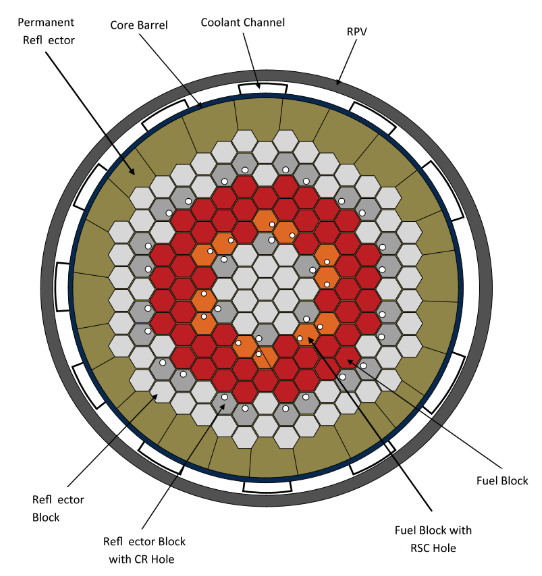
\includegraphics[width=\linewidth]{figures/radial-layout.png}
	% 		\caption{XY-plane.}
	% 	\end{subfigure}
	% 	\begin{subfigure}[t]{0.4\textwidth}
	% 		\centering
	% 		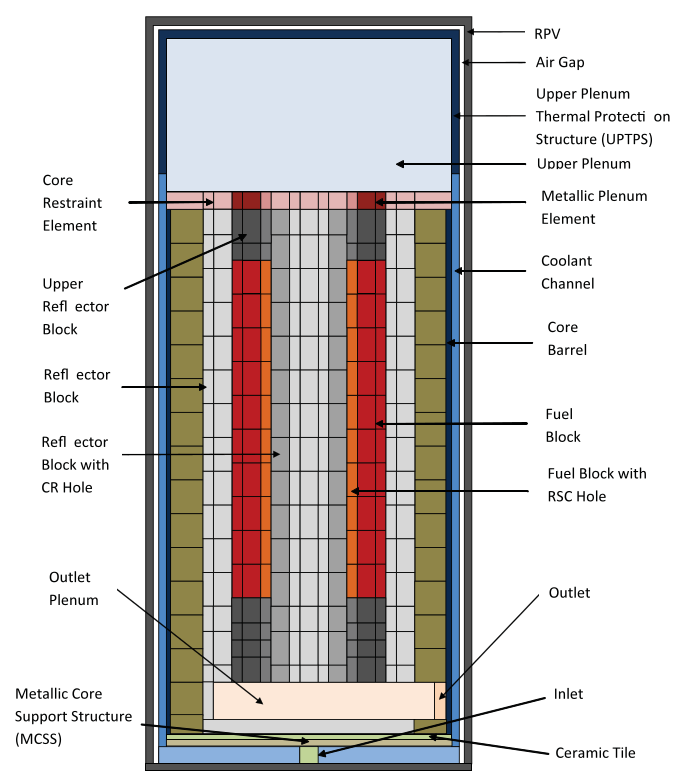
\includegraphics[width=\linewidth]{figures/axial-layout.png}
	% 		\caption{YZ-plane.}
	% 	\end{subfigure}
	% 	\hfill
	% 	\caption{MHTGR reactor layout.}
	% 	\label{fig:layout}
	% \end{figure}

	% \begin{figure}[htbp!]
	% 	\centering
	% 	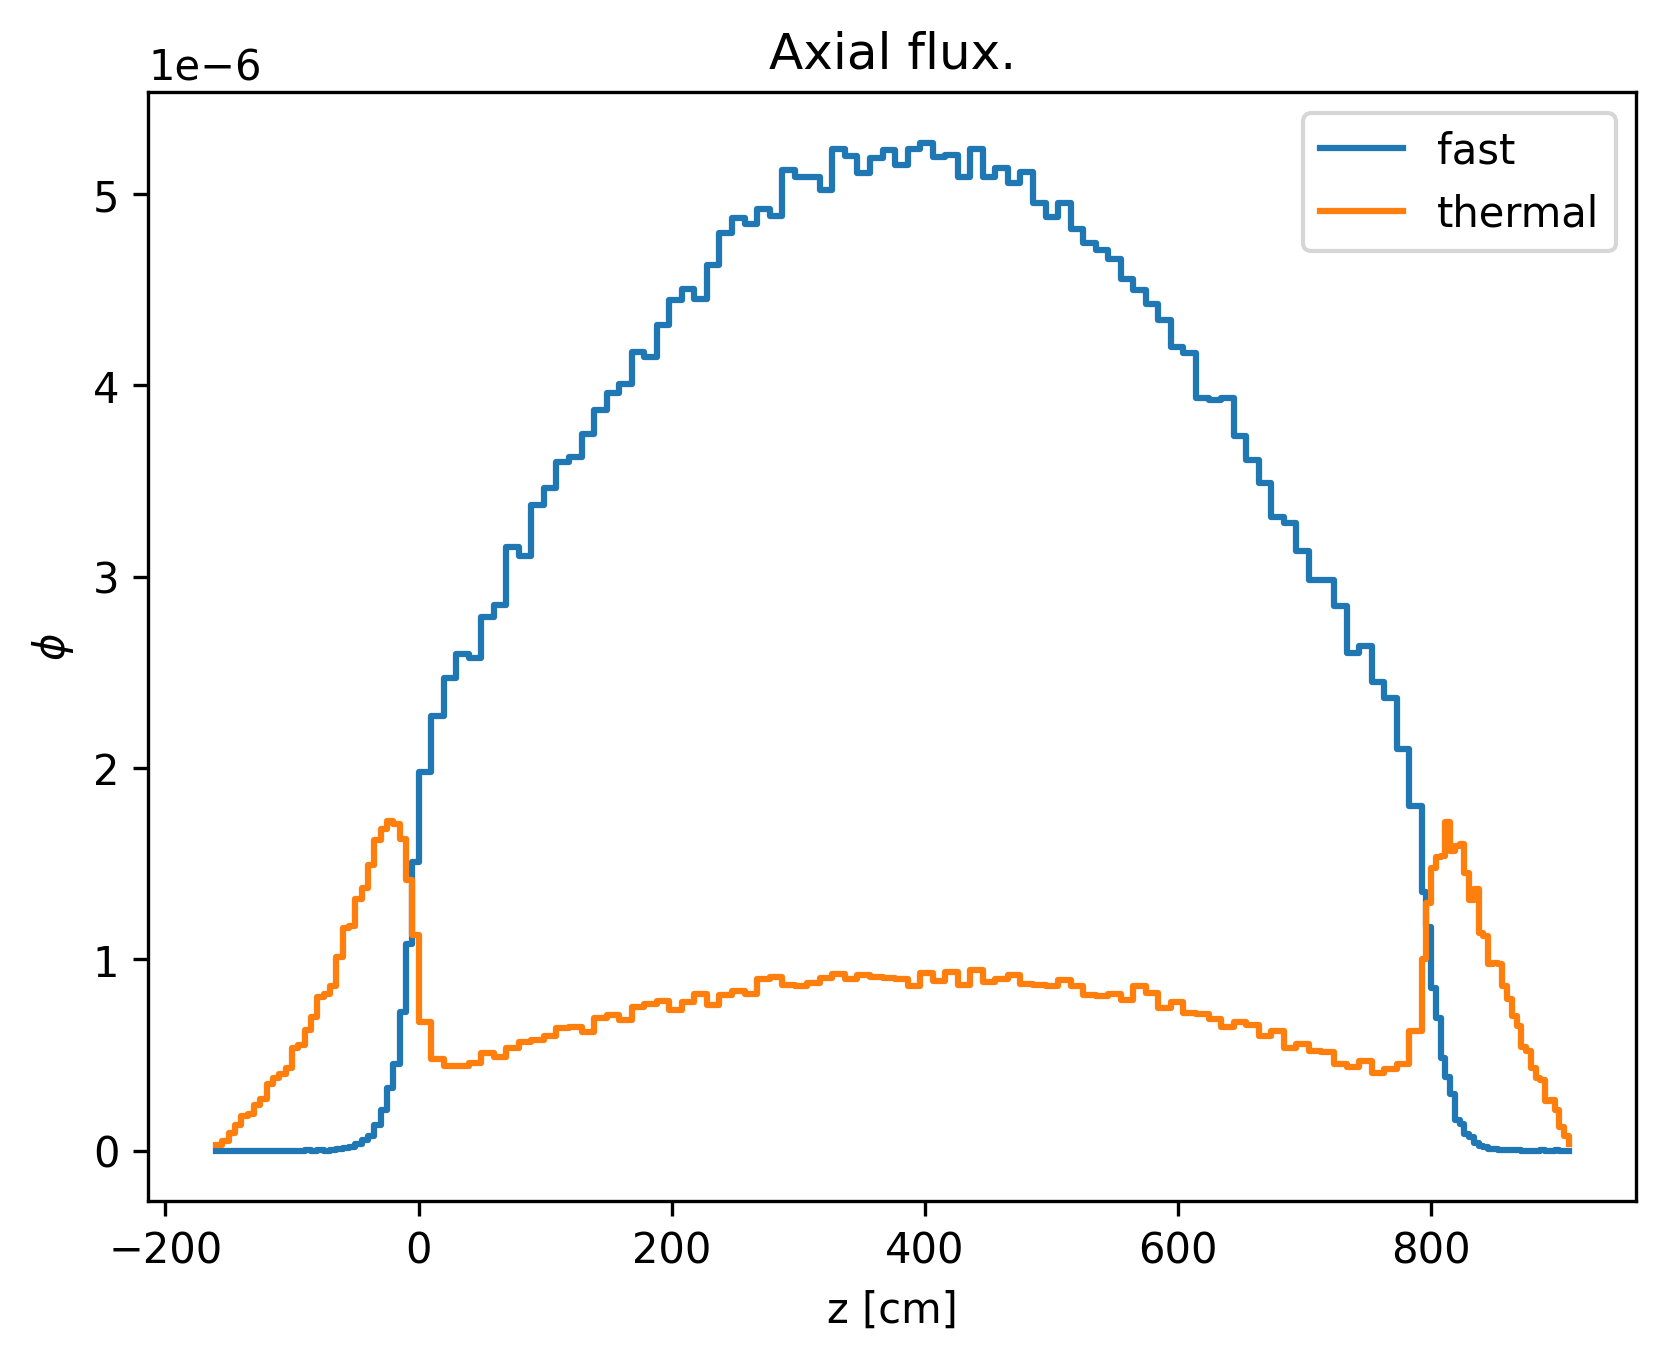
\includegraphics[width=0.6\linewidth]{figures/axial1.png}
	% 	\hfill
	% 	\caption{Neutron flux on the specified fuel channel.}
	% 	\label{fig:axial}
	% \end{figure}
